\chapter{Fundamentos}
Este capitulo apresenta os fundamentos do trabalho. Segundo \citeonline{einstein1905}, a luz tem natureza quantica.
\section{Equacoes basicas}
A energia de repouso vale
\begin{equation}
E = mc^2
\end{equation}
e a segunda relacao e
\begin{equation}
\int_0^1 x^2\,dx = \frac{1}{3}
\end{equation}
\section{Figura de exemplo}
A Figura~\ref{fig:um} mostra um desenho vetorial simples.
\begin{figure}[htb]
\caption{Desenho vetorial um}\label{fig:um}
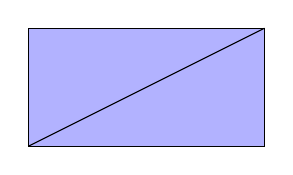
\begin{tikzpicture}\draw[fill=blue!30] (0,0) rectangle (3,1.5);\draw (0,0) -- (3,1.5);\end{tikzpicture}
\end{figure}
\begin{table}[htb]
\caption{Tabela de resultados um}
\begin{tabular}{lcc}\hline
Amostra & Massa & Volume \\ \hline
alfa & 12 & 3 \\
beta & 15 & 4 \\ \hline
\end{tabular}
\end{table}
